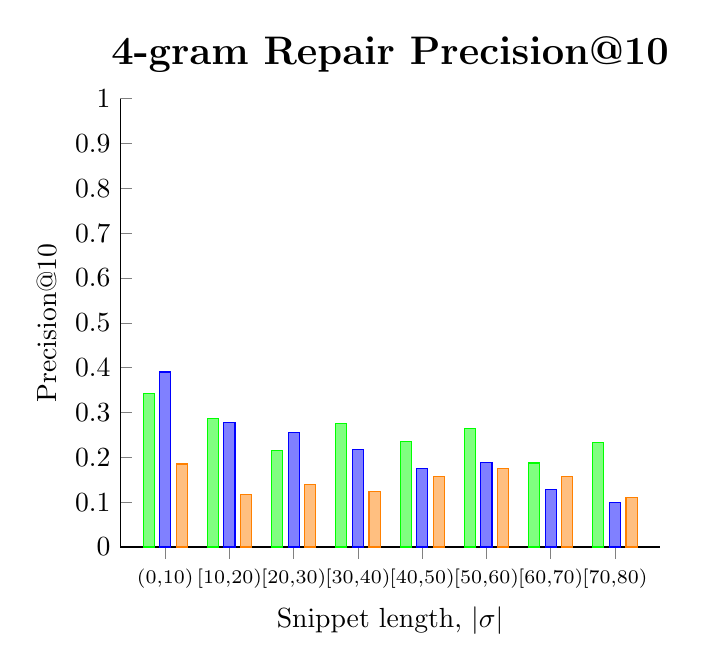
\begin{tikzpicture}
  \begin{axis}[
  xlabel={Snippet length, $|\sigma|$},
  ylabel={Precision@10},
  title={\Large\textbf{4-gram Repair Precision@10}},
  ybar,
  axis lines*=left,
  xtick={0, 10, 20, 30, 40, 50, 60, 70},
  ytick={0, 0.1, 0.2, 0.3, 0.4, 0.5, 0.6, 0.7, 0.8, 0.9, 1.0},
  xticklabels={{(}0{,}10{)}, {[}10{,}20{)}, {[}20{,}30{)}, {[}30{,}40{)}, {[}40{,}50{)}, {[}50{,}60{)}, {[}60{,}70{)}, {[}70{,}80{)}},
  x tick label style={font=\scriptsize},
  ymax=1.0,
  ymin=0.0,
  bar width=4pt,
  ]
  \addplot[green, fill=green!50] coordinates { (0, 0.34210526315789475) (10, 0.28762541806020064) (20, 0.2150170648464164) (30, 0.27586206896551724) (40, 0.23529411764705882) (50, 0.2638888888888889) (60, 0.1875) (70, 0.23295454545454544) };
  \addplot[blue, fill=blue!50] coordinates { (0, 0.3904761904761905) (10, 0.27759197324414714) (20, 0.2560553633217993) (30, 0.2179930795847751) (40, 0.17465753424657535) (50, 0.18811881188118812) (60, 0.1292517006802721) (70, 0.1) };
  \addplot[orange, fill=orange!50] coordinates { (0, 0.18518518518518517) (10, 0.11643835616438356) (20, 0.14) (30, 0.12337662337662338) (40, 0.15789473684210525) (50, 0.175) (60, 0.15789473684210525) (70, 0.1111111111111111) };
  \end{axis}
\end{tikzpicture}